\documentclass{standalone}
\usepackage{tikz}
\usepackage{ctex,siunitx}
\setCJKmainfont{Noto Serif CJK SC}
\usepackage{tkz-euclide}
\usepackage{amsmath}
\usepackage{wasysym}
\usetikzlibrary{patterns, calc}
\usetikzlibrary {decorations.pathmorphing, decorations.pathreplacing, decorations.shapes,}
\begin{document}
\small
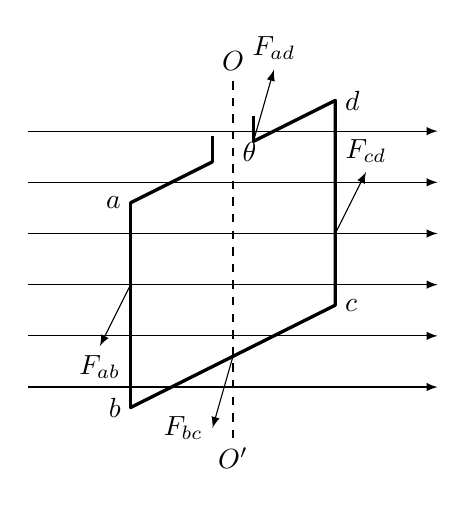
\begin{tikzpicture}[>=latex,scale=1.3]
  \foreach \x in {-1,-.5,...,1.5}
  {
    \draw[->](-2,\x)--(2,\x);
  }
  \draw[dashed](0,-1.5)node[below]{$O'$}--(0,2)node[above]{$O$};
  \tkzDefPoints{-1/.8/a, 1/1.8/d, -1/-1.2/b}
  \tkzDefPointsBy[translation= from a to b](d){c}
  \tkzDrawSegments[very thick](a,b b,c c,d)
  \tkzDefPointWith[linear, K=.4](a,d)\tkzGetPoint{a'}
  \tkzDefPointWith[linear, K=.6](a,d)\tkzGetPoint{d'}
  \tkzDrawSegments[very thick](a,a' d,d')
  \tkzLabelPoints[left](a,b)
  \tkzLabelPoints[right](c,d)
  \draw[very thick](a')--+(0,.25);
  \draw[very thick](d')--+(0,.25);
  \draw[->](d')--+(0.2,.7)node[above]{$F_{ad}$};
  \draw[->](1,0.5)--+(0.3,.6)node[above]{$F_{cd}$};
  \draw[->](-1,0)--+(-0.3,-.6)node[below]{$F_{ab}$};
  \draw[->](0,-.7)--+(-0.2,-.7)node[left]{$F_{bc}$};
  \node at (0,1.3)[right]{$\theta$};
\end{tikzpicture}
\end{document}